\subsection{Preprocessing}\label{sec:preprocessing}

Main preprocessing is done in \soft{HALFpipe} with \soft{fMRIPrep}, which performs a consensus of preprocessing steps required for any fMRI study \parencite{esteban2019a}. Consensus steps for structural images include skull stripping, tissue segmentation, and spatial normalization. Consensus steps for functional images include motion correction, slice time correction, susceptibility distortion correction, coregistration, and spatial normalization (Figure 1).

\soft{HALFpipe} defines standard space as the \term{MNI152NLin2009cAsym} template, which is the most current and detailed template available (Horn 2016a). Note that the standard space template is not user-configurable, so that any outputs generated by one version of \soft{HALFpipe} can be easily compared to outputs generated by another version of \soft{HALFpipe}.

Once the fMRI data have been processed with \soft{fMRIPrep} and resampled into standard space, \soft{HALFpipe} implements a number of additional preprocessing steps for denoising, filtering, and harmonizing the functional data (see also Figure 1):

\begin{enumerate}[leftmargin=*]

\item

\soft{ICA-AROMA} is an algorithm based on independent component analysis. It classifies components into those that contain signal and those that are noise \parencite{pruim2015}. To accomplish this, \soft{ICA-AROMA} relies on reference templates defined in \term{MNI152NLin6Asym} space, which is different from the standard space template \term{MNI152NLin2009cAsym} that is used by \soft{fMRIPrep}. To allow \soft{ICA-AROMA} to run, it is thus necessary to provide the preprocessed image not just in the default template space, but also in the one required by \soft{ICA-AROMA}. By default, \soft{fMRIPrep} will estimate a second normalization to this other template, apply it to the fMRI image in native space, and run \soft{ICA-AROMA} on the resulting image \parencite{ciric2021}. This approach effectively doubles the processor time spent on spatial normalization, and may require manually checking both spatial registrations.

To avoid this considerable effort, \soft{HALFpipe} implements a different approach by using an existing warp between the two standard template spaces \parencite{horn2016c}. This predefined warp is concatenated with the normalization that was already estimated by \soft{fMRIPrep}, and then a second round of resampling is performed with \soft{fMRIPrep}'s \code{bold\_std\_trans\_wf} This way, only the resampling step needs to be run twice.

Finally, \soft{ICA-AROMA} is run on the resulting fMRI image in \term{MNI152NLin6Asym} space using \soft{fMRIPrep}'s \code{ica\_aroma\_wf} workflow, which also includes spatial smoothing fixed to a 6 mm FWHM smoothing kernel. The resulting classifications are kept for step~\ref{itm:aroma}.

\item

\soft{HALFpipe} implements spatial smoothing using \soft{AFNI}'s \soft{3dBlurToFWHM} \parencite{friedman2006}. Each voxel's signal is averaged with the signal of surrounding voxels weighted by an isotropic gaussian kernel. At the edges of the brain, this kernel may include non-brain voxels, so smoothing is constrained by the brain mask. This is equivalent to the procedure in the \term{Minimal Preprocessing Pipelines for the Human Connectome Project} \parencite{glasser2013}. In addition, \soft{3dBlurToFWHM} estimates the smoothness of the resulting image, and iteratively decreases the amount of smoothing so that the resulting smoothness matches the user setting. This way, differences in the intrinsic smoothness between datasets (e.g., due to different voxel sizes) can be harmonized.

\item\label{itm:grandmean}

Grand mean scaling sets the image mean, defined as the within-scan mean across all voxels and time points, to a predefined value. The grand mean is closely related to scanner parameters such as RF power or amplifier gain but not to neural mechanisms \parencite{gavrilescu2002}. Adjusting the grand mean via scaling makes analysis results more interpretable and comparable across subjects, sessions, and sites. The scaling factor is calculated based on the masked functional image, and applied to both the fMRI data and the confound time series extracted by \soft{fMRIPrep}.

\item\label{itm:aroma}

If selected, the previously estimated \soft{ICA-AROMA} noise components are removed from the smoothed and grand-mean-scaled fMRI data. This is done in a non-aggressive way to minimize removing variance that is shared between signal and noise components. \soft{ICA-AROMA} implements this step using the \soft{FSL} command \soft{fsl\_regfilt}, which calculates an ordinary least squares regression for each voxel, where the design matrix includes both the signal and the noise components as regressors. This means that the resulting regression weights reflect the unique variance of the noise components (and not the shared variance with signal components). Then, the noise component regressors are multiplied by their regression weights and these products are added together to yield one time series of the noise. Subtracting the noise from the voxel time series yields a denoised time series (the regression residuals). This step is done using a custom re-implementation of \soft{fsl\_regfilt} in \soft{HALFpipe} using \soft{Numpy} \parencite{harris2020}.

\item\label{itm:tempfilt}

Temporal filtering can be selected to remove low-frequency drift via a high-pass filter, high-frequency noise via a low-pass filter, or both at the same time using a band-pass filter. \soft{HALFpipe} implements two approaches to temporal filtering, a frequency-based approach \parencite{jo2013} and a Gaussian-weighted approach \parencite{marchini2000}. The frequency-based temporal filter is very exact in selecting frequencies to be kept or removed, and is commonly used to calculate fractional Amplitude of Low Frequency Fluctuations (fALFF) and Regional Homogeneity (ReHo). The Gaussian-weighted temporal filter is the default used by \soft{FSL Feat} \parencite{jenkinson2012} and may have fewer edge effects at the start and end of the time series. However, its spectrum also has a more gradual roll-off, meaning that it will be less aggressive in removing frequencies close to the chosen cutoff value.

\end{enumerate}

Importantly, \soft{HALFpipe} runs \soft{fMRIPrep} with small modifications. For instance, we disabled \soft{fMRIPrep}’s experimental susceptibility distortion correction in the absence of field maps, because it is not yet validated. Further, \soft{HALFpipe} suggests default settings for each preprocessing step, which are outlined in Table~\ref{table:settings}. Note that some are selected based on best-practices in the field (i.e., band-pass temporal filter for ALFF and ReHo), whereas most default settings can be adjusted by the user. Last, \soft{HALFpipe} does not output preprocessed and normalized functional images by default, because they use a lot of disk space. However, in the user interface users can manually choose to output a preprocessed functional image with their choice of preprocessing settings.

\begin{figure}[!tb]
    \begin{adjustwidth}{-2.4cm}{}
        \hsize=\linewidth%
        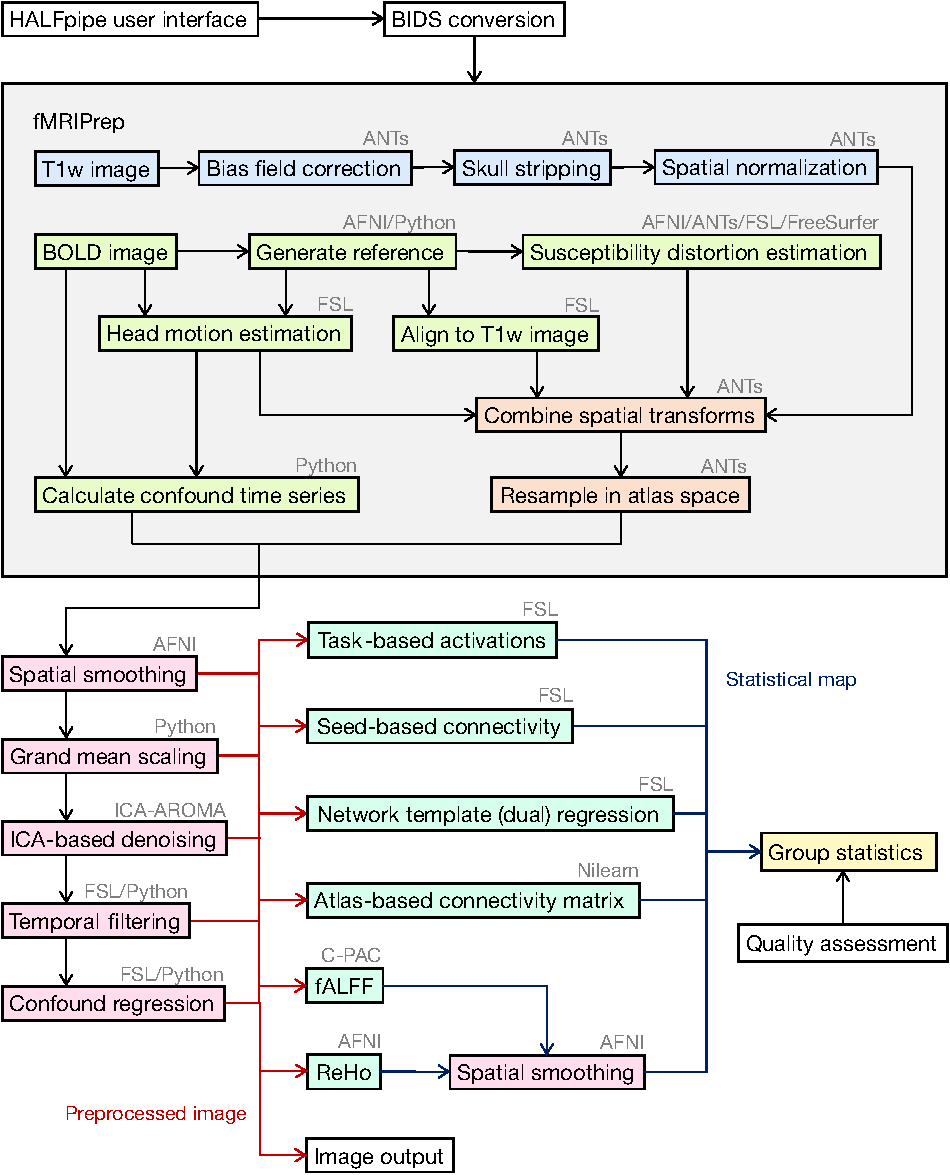
\includegraphics[width=\linewidth]{fig/workflow/workflow-crop}
        \caption{\textbf{\soft{HALFpipe} workflow.} \soft{HALFpipe} is configured in a user interface where the user is asked a series of questions about their data and the processing steps to perform. Data is then converted to BIDS format \parencite{gorgolewski2016b} to allow standardized processing (white). After minimal preprocessing of the structural (blue) and functional (green and orange) data with \soft{fMRIPrep} \parencite{esteban2019a}, additional preprocessing steps can be selected (red). Using the preprocessed data, statistical maps can be calculated during feature extraction (turquoise). Finally, group statistics can be performed (yellow). Note that not all preprocessing steps are available for each feature, as is outlined in Table~\ref{table:settings}. The diagram omits this information to increase visual clarity.}\label{fig:workflow}
  \end{adjustwidth}
\end{figure}
